%----------------------------------------
% IT IS RECOMMENDED TO USE AUTOLATEX FOR
% COMPILING THIS DOCUMENT.
% http://www.arakhne.org/autolatex
%----------------------------------------

\documentclass[english,nodocumentinfo,nopubpage]{utbmciadreport}

% The TeX code is entering with UTF8
% character encoding (Linux and MacOS standards)
\usepackage[utf8]{inputenc}
\usepackage{fancyhdr}
\usepackage{../common/sarl-colorized-listing}


\graphicspath{{./}}

\declaredocument{Introduction to SARL}{Tutorial Session \#2}{UTBM-INFO-AI51-TU2}

\addauthorvalidator*[St\'ephane Galland]{St{\'e}phane}{Galland}{Teacher}

\updateversion{1.0}{\makedate{20}{03}{2023}}{First release on Github}{\upmpublic}

\begin{document}

\section{Goal of this Tutorial Session}

The goal of this tutorial session is to introduce the basics concepts of agent-oriented programming with SARL.
The general goal of the tutorial is to create a simple software that is implementing the "Prey-Predator" problem.

The Prey/ Predators problem is a pursuit game, including four predators and one prey. Initially, they are scattered randomly on a field represented as a bi-dimensional grid, and the goal of the game consists in the capture of the prey by the predators as shown in Figure \ref{fig1}.

\begin{figure}{ht}
	\centering
	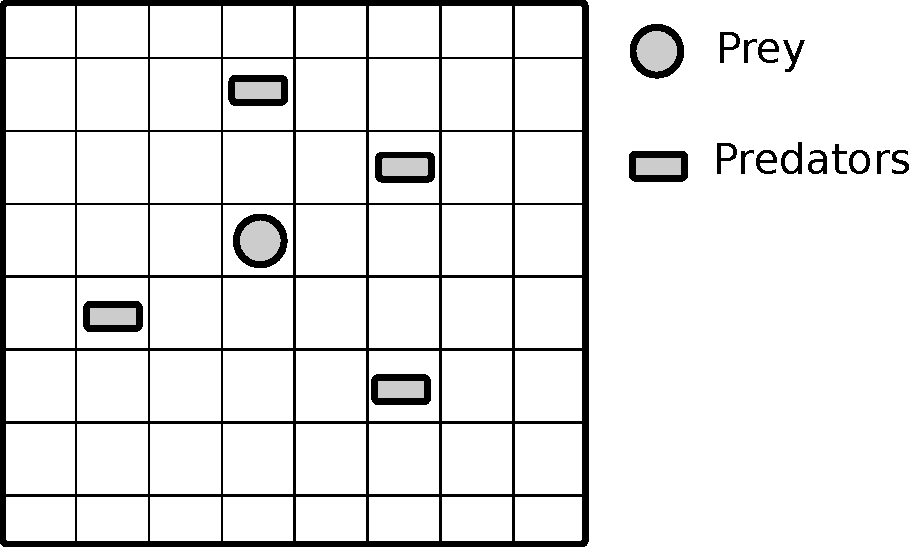
\includegraphics[width=.6\linewidth]{fig1}
	\caption{Grid environment for the Prey-Predator game}
	\label{fig1}
\end{figure}

The game starts with the move of the agents on the grid in an horizontal or vertical way. The prey moves in a random way. At each step, it chooses haphazardly a direction. If the prey goes out the game field, it wins the match against its hunters. A predator can perceive the prey only if it is in its perception scope. Figure \ref{fig2} shows the predator's perception scope which corresponds to a distance of two units (two juxtaposed boxes). When a predator knows the prey's position, it moves on the field toward the prey in order to reach the position determined by its role. This role is to occupy the position at the south, the east, the west or the north of the prey. When it doesn't know this position, it moves randomly on the field. Two means are used by a predator to know the prey's position:
\begin{itemize}
	\item The prey stays in its perception scope and hence it is visible to the predator.
	\item The predator asks its colleagues for the prey position 
\end{itemize}

\begin{figure}{ht}
	\centering
	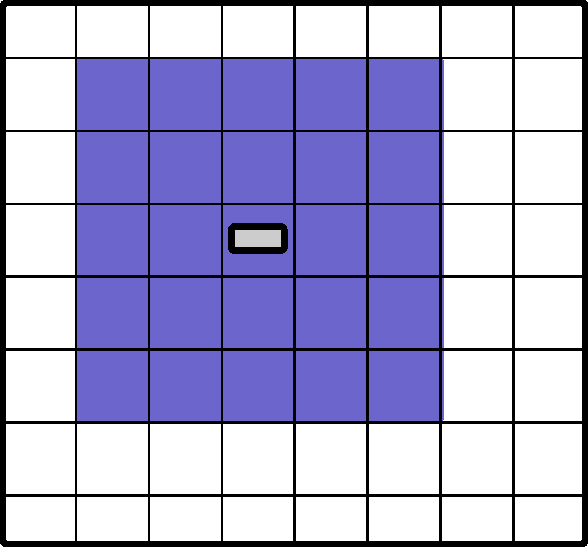
\includegraphics[width=.6\linewidth]{fig2}
	\caption{Perception area of the Predators}
	\label{fig2}
\end{figure}

\section{Work to be Done during the Tutorial Session}

The following sections describe the work to be done during this tutorial session. Before running the game, the components of the software must be implemented: grid environment, and the prey and predator agents.

\subsection{Grid Environment}

The grid environment is an entity that must contains the bodies of the agents (the prey and the predator). The grid environment is based on a data structure that is a 2-dimension array of bodies. Each cell of the grid could contain maximum 1 body.

The steps to be done:
\begin{enumerate}[a)]
\item Create a class \code{Body} using the object-oriented programming paradigm in SARL ou Java that represents a body. A body object has the following properties:
	\begin{itemize}
		\item \code{id} : an UUID that must have the same value as the identifier of the associated agent.
		\item \code{isPrey} : a boolean flag indicating if the body is for the prey or a predactor.
		\item \code{x, y} : two attributes representing the position of the body in the grid.
	\end{itemize}
\item Create a class \code{GridEnvironment} that is representing the grid environment. It must contains:
	\begin{itemize}
	\item \code{matrix} : a 2-dimension grid of bodies.
	\item \code{getPerception(id : UUID) : List<Body>} that computes the list of bodies that is in the field of perception of the body/agent with the given identifier.
	\item \code{move(id : UUID, dx : int, dy : int) : boolean} that moves the body with the given identifier in the direction represented by the vector $(dx,dy)$. The values of this vector must be in $[-1;1]$. This function replies \code{true} if the new position of the body is outside the grid.
\end{itemize}
\end{enumerate}

\section{Perception Event}

In order to give to the agents their perception, the most simple mean is to define a dedicated event.
\begin{enumerate}[a)]
	\item Define the event \code{Perception}.
	\item Add in the event an attribute that represents the list of bodies in the field of view of an agent : \code{List<Body>}
\end{enumerate}

\section{Move Capacity}

In order to give to the agents the capability to move in the grid, the best approach is to define a dedicated known-how using the concepts of capacity and skill:
\begin{enumerate}[a)]
	\item Define the capacity \code{MoveInGrid}.
	\item Add in the function in the capacity for moving the agent.
	\item Define the skill \code{MoveInGridImpl} that implements the capacity \code{MoveInGrid}, and contains an attribute that is a reference to the grid environment.
	\item Define a constructor for the \code{MoveInGridImpl} skill for initialized the attribute.
\end{enumerate}

\subsection{Prey Agent}

Given the template of code for the prey agent:
\begin{lstlisting}
	agent Prey {
		uses MoveInGrid
		on Initialize {
			setSkill(new MoveInGridImpl(occurrence.parameters.get(0) as GridEnvironment))
		}
		on Perception {
			
		}
	}
\end{lstlisting}

\begin{enumerate}[a)]
	\item Define the prey behavior and write it inside \code{on Perception}. This behavior must read the prey's perception from the \code{Perception} event, using the keyword \code{occurrence}. The last instruction to be run in the behavior must be a call to the function that is defined in the \code{MoveInGrid} capacity.
\end{enumerate}

\subsection{Predator}

Given the template of code for the predator agent:
\begin{lstlisting}
	agent Predator {
		uses MoveInGrid
		on Initialize {
			setSkill(new MoveInGridImpl(occurrence.parameters.get(0) as GridEnvironment))
		}
		on Perception {
			
		}
	}
\end{lstlisting}

\begin{enumerate}[a)]
	\item Define the pedator behavior and write it inside \code{on Perception}. This behavior must read the predator's perception from the \code{Perception} event, using the keyword \code{occurrence}. The last instruction to be run in the behavior must be a call to the function that is defined in the \code{MoveInGrid} capacity.
\end{enumerate}

\subsection{Run the game}

For running the game, we have to create a "main" agent that is in charge of creating the grid environment and spawning the agents:
\begin{enumerate}[a)]
	\item Define the \code{Main} agent.
	\item In the initialization code, create the instance of the grid environment with the minimum size $7x7$.
	\item In the initialization code, spawn the Prey agent with the grid environment as argument.
	\item In the initialization code, spawn the 4 Predator agents with the grid environment as argument.
\end{enumerate}

\textbf{\textcolor{red}{CHALLENGE: Determine and provide the implementation of the functions, \code{on} event handlers and events that must be implemented to create the infinite loop for running the agents. There is no strict guideline on this point. Details and guidelines are in the slides of the lecture.}}

\subsection{Graphical User Interface (Optional)}

For seeing the state of the grid environment during the game, you could implement a graphical user interface (using Swing or any other Java-based library).

\end{document}
